\begin{frame}{The $\Upsilon$ fit model}
\setlength{\unitlength}{1mm}
\begin{columns}[T]
\column{.5\textwidth}
\resizebox{\textwidth}{!}{
  \begin{picture}(75,60)
    \put(0,0){
      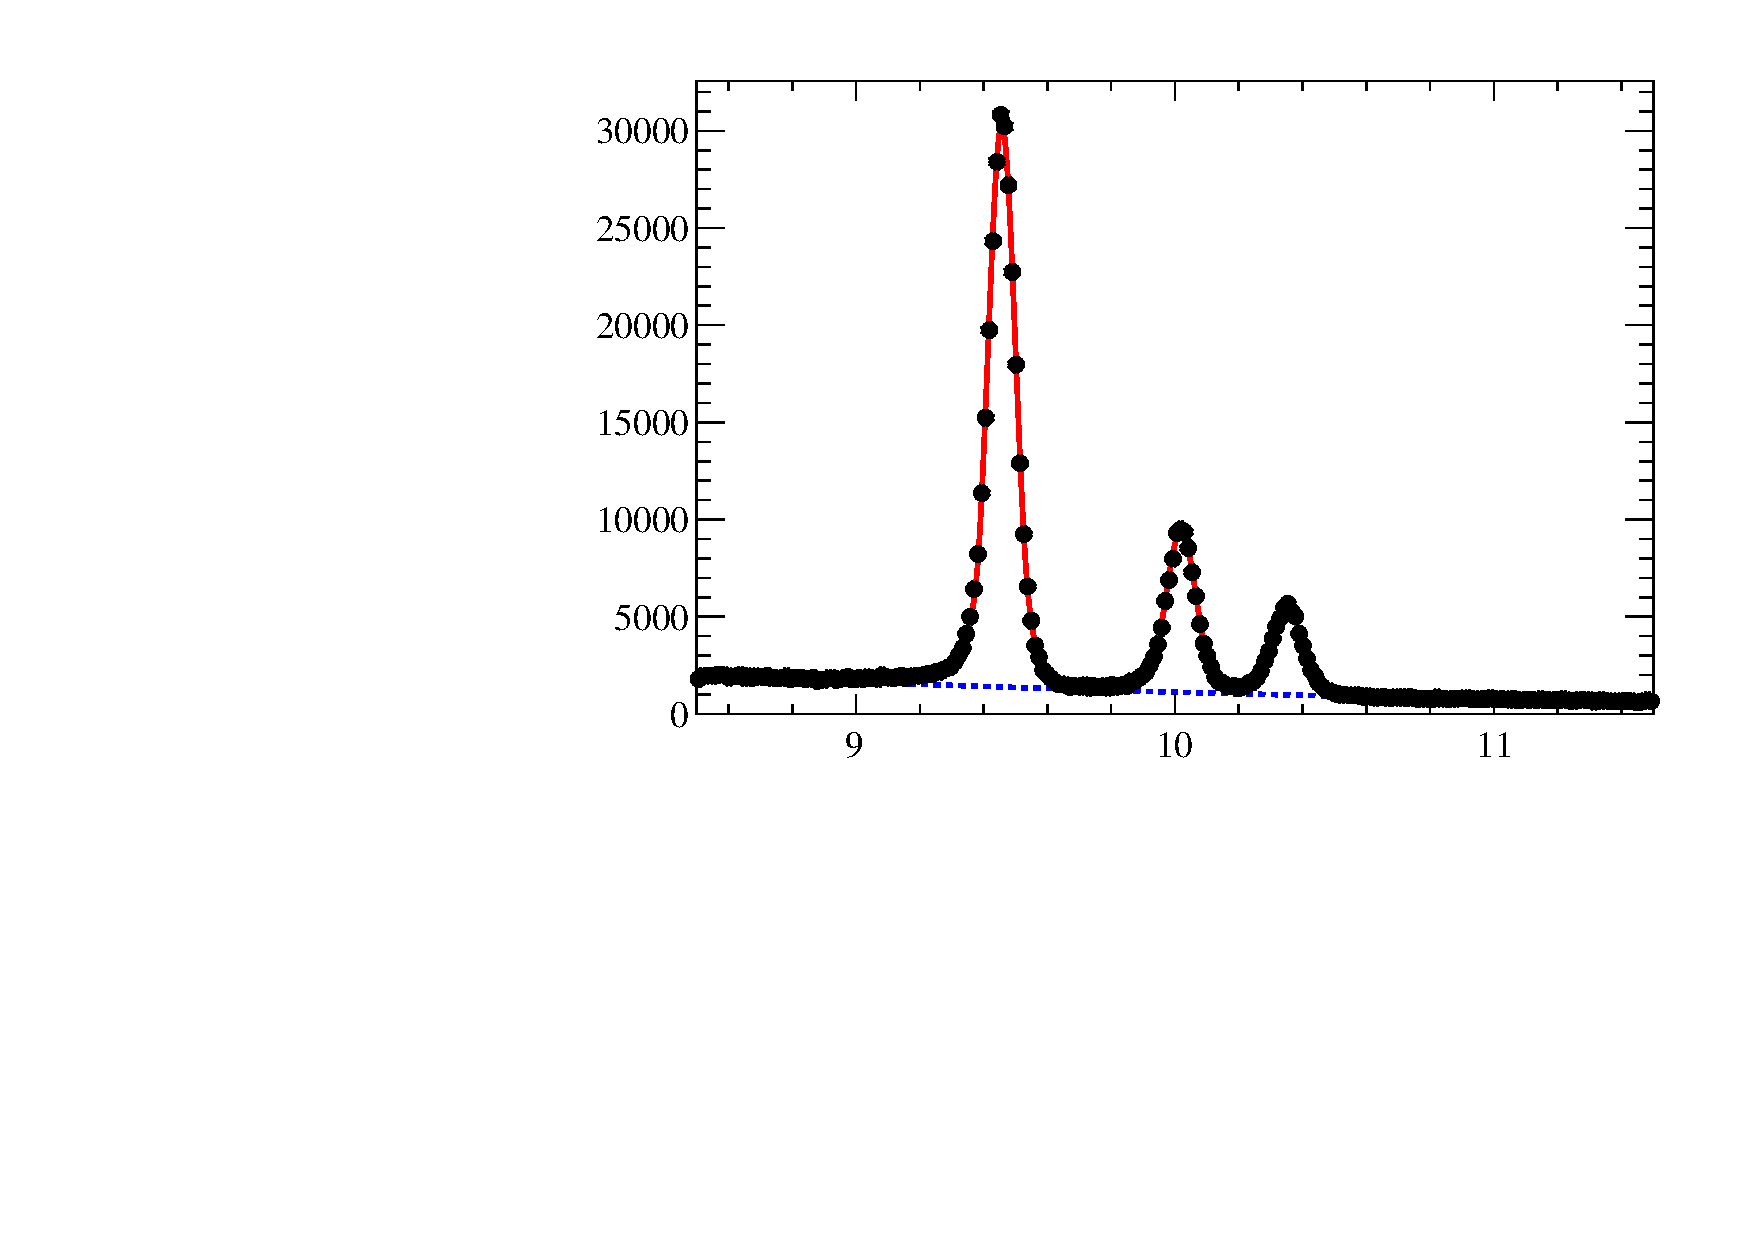
\includegraphics[width=75mm, height=60mm]{ups_f2011_6_40}
    }
    \put(0,18){\small \begin{sideways}Candidates/(40\mevcc)\end{sideways}}
    \put(25, 0){$m_{\mumu} \left[\gevcc\right]$}
    \put(45,45){\sqs = 7 \tev}
    \put(35,38){$6 < p_T^{\mumu} < 12 \gevc$}
    
    \put(18,50){\Y1S}
    \put(40,25){\Y2S}
    \put(50,20){\Y3S}
    % \graphpaper[5](0,0)(75, 60)
  \end{picture}
}

\column{.5\textwidth}
\resizebox{\textwidth}{!}{
\begin{tabular}{lrr}\toprule
 & \multicolumn{2}{c}{$\mumu$ transverse momentum intervals, \gevc}\\
 & \multicolumn{2}{c}{6 -- 40}\\
\cmidrule(r){2-3}
 & \multicolumn{1}{c}{\sqs = 7\tev} & \multicolumn{1}{c}{\sqs = 8\tev}\\
\midrule
$N_{\Y1S}$ & 283,300 $\pm$ 600 & 659,600 $\pm$ 900\\
$N_{\Y2S}$ & 87,500 $\pm$ 400 & 203,300 $\pm$ 600\\
$N_{\Y3S}$ & 50,420 $\pm$ 290 & 115,300 $\pm$ 400015\\
\bottomrule
\end{tabular}
} % scalebox
\end{columns}

\bigskip

\begin{itemize}
\item 3 Double Crystal Ball functions for signal yields. Side band parameters are fixed
from simulation.
\item Exponential function for combinatorial background.
\end{itemize}


\end{frame}

